\documentclass{standalone}
\usepackage{tikz}
\usetikzlibrary{patterns, positioning}


\begin{document}
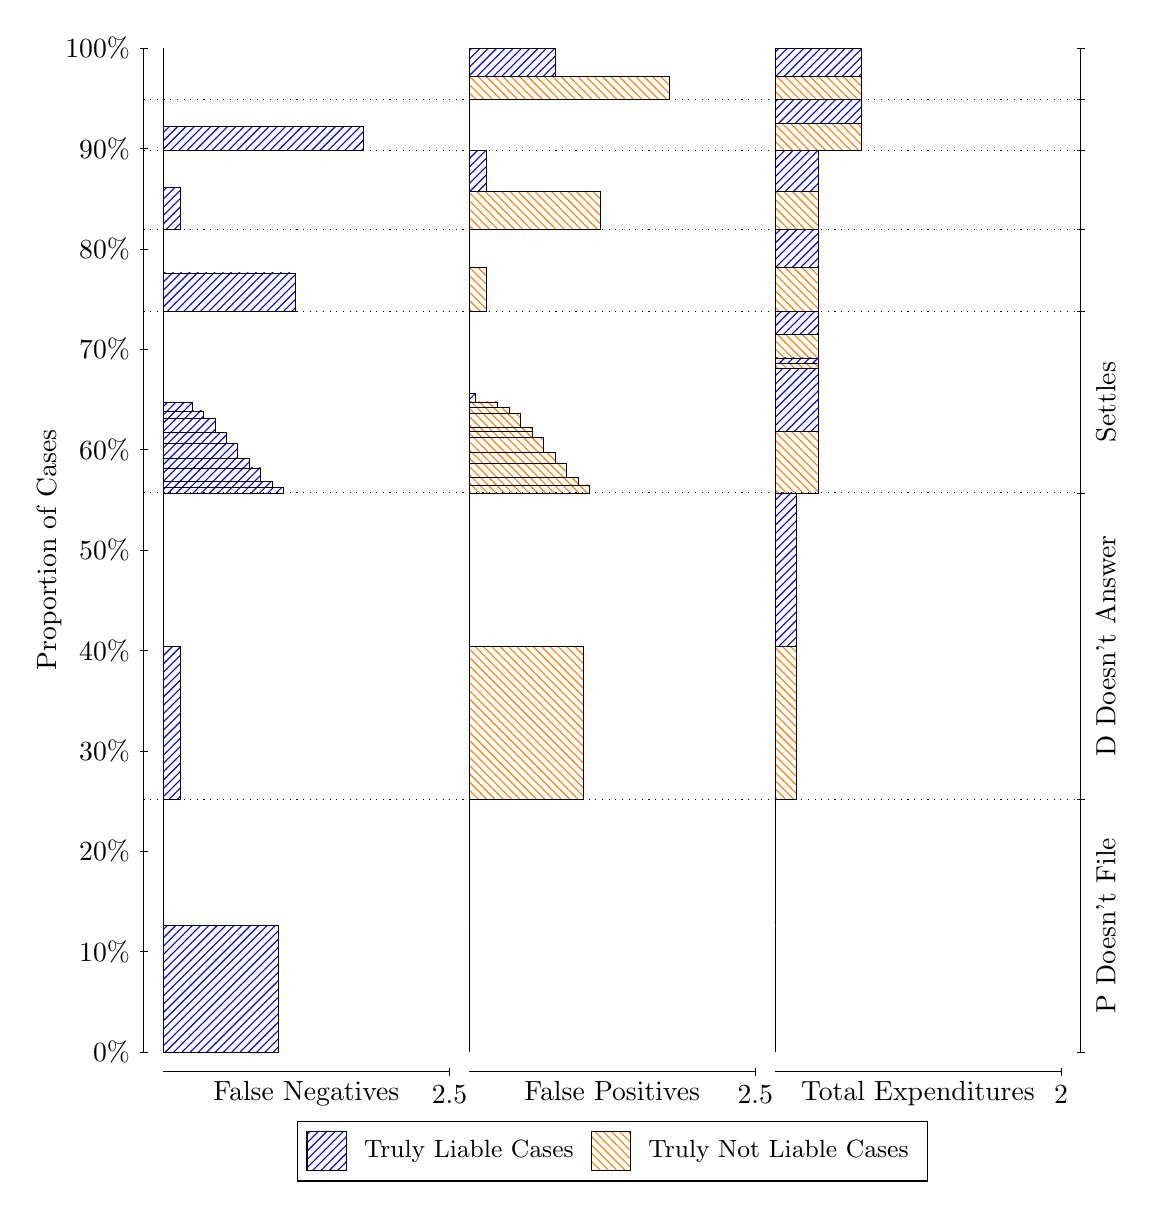
\begin{tikzpicture}
\draw[black, very thin] (1.5,1.75) -- (1.5,14.5);
\node[rotate=90, text=black, anchor=center] at (0.3, 8.125) {Proportion of Cases};
\draw[black, very thin] (1.45,1.75) -- (1.55,1.75);
\node[text=black, anchor=east] at (1.45, 1.75) {0\%};
\draw[black, very thin] (1.45,3.025) -- (1.55,3.025);
\node[text=black, anchor=east] at (1.45, 3.025) {10\%};
\draw[black, very thin] (1.45,4.3) -- (1.55,4.3);
\node[text=black, anchor=east] at (1.45, 4.3) {20\%};
\draw[black, very thin] (1.45,5.575) -- (1.55,5.575);
\node[text=black, anchor=east] at (1.45, 5.575) {30\%};
\draw[black, very thin] (1.45,6.85) -- (1.55,6.85);
\node[text=black, anchor=east] at (1.45, 6.85) {40\%};
\draw[black, very thin] (1.45,8.125) -- (1.55,8.125);
\node[text=black, anchor=east] at (1.45, 8.125) {50\%};
\draw[black, very thin] (1.45,9.4) -- (1.55,9.4);
\node[text=black, anchor=east] at (1.45, 9.4) {60\%};
\draw[black, very thin] (1.45,10.675) -- (1.55,10.675);
\node[text=black, anchor=east] at (1.45, 10.675) {70\%};
\draw[black, very thin] (1.45,11.95) -- (1.55,11.95);
\node[text=black, anchor=east] at (1.45, 11.95) {80\%};
\draw[black, very thin] (1.45,13.225) -- (1.55,13.225);
\node[text=black, anchor=east] at (1.45, 13.225) {90\%};
\draw[black, very thin] (1.45,14.5) -- (1.55,14.5);
\node[text=black, anchor=east] at (1.45, 14.5) {100\%};

\draw[black, very thin] (13.4,1.75) -- (13.4,14.5);
\draw[black, very thin] (13.35,1.75) -- (13.45,1.75);
\node[anchor=west] at (13.35, 1.75) {};
\draw[black, very thin] (13.35,4.958) -- (13.45,4.958);
\node[anchor=west] at (13.35, 4.958) {};
\draw[black, very thin] (13.35,8.8516) -- (13.45,8.8516);
\node[anchor=west] at (13.35, 8.8516) {};
\draw[black, very thin] (13.35,11.157) -- (13.45,11.157);
\node[anchor=west] at (13.35, 11.157) {};
\draw[black, very thin] (13.35,12.2) -- (13.45,12.2);
\node[anchor=west] at (13.35, 12.2) {};
\draw[black, very thin] (13.35,13.203) -- (13.45,13.203);
\node[anchor=west] at (13.35, 13.203) {};
\draw[black, very thin] (13.35,13.85) -- (13.45,13.85);
\node[anchor=west] at (13.35, 13.85) {};
\draw[black, very thin] (13.35,14.5) -- (13.45,14.5);
\node[anchor=west] at (13.35, 14.5) {};

\draw[black, very thin, pattern color=blue, pattern=north east lines] (1.75,1.75) rectangle (3.2033,3.354);
\draw[black, very thin, pattern color=orange, pattern=north west lines] (1.75,3.354) rectangle (1.75,4.958);
\draw[black, very thin, pattern color=blue, pattern=north east lines] (1.75,4.958) rectangle (1.968,6.9048);
\draw[black, very thin, pattern color=orange, pattern=north west lines] (1.75,6.9048) rectangle (1.75,8.8516);
\draw[black, very thin, pattern color=blue, pattern=north east lines] (1.75,8.8516) rectangle (3.276,8.9172);
\draw[black, very thin, pattern color=blue, pattern=north east lines] (1.75,8.9172) rectangle (3.1307,8.9943);
\draw[black, very thin, pattern color=blue, pattern=north east lines] (1.75,8.9943) rectangle (2.9853,9.1671);
\draw[black, very thin, pattern color=blue, pattern=north east lines] (1.75,9.1671) rectangle (2.84,9.2876);
\draw[black, very thin, pattern color=blue, pattern=north east lines] (1.75,9.2876) rectangle (2.6947,9.4813);
\draw[black, very thin, pattern color=blue, pattern=north east lines] (1.75,9.4813) rectangle (2.5493,9.6179);
\draw[black, very thin, pattern color=blue, pattern=north east lines] (1.75,9.6179) rectangle (2.404,9.8009);
\draw[black, very thin, pattern color=blue, pattern=north east lines] (1.75,9.8009) rectangle (2.2587,9.8926);
\draw[black, very thin, pattern color=blue, pattern=north east lines] (1.75,9.8926) rectangle (2.1133,10.003);
\draw[black, very thin, pattern color=orange, pattern=north west lines] (1.75,10.003) rectangle (1.75,11.157);
\draw[black, very thin, pattern color=blue, pattern=north east lines] (1.75,11.157) rectangle (3.4213,11.644);
\draw[black, very thin, pattern color=orange, pattern=north west lines] (1.75,11.644) rectangle (1.75,12.2);
\draw[black, very thin, pattern color=blue, pattern=north east lines] (1.75,12.2) rectangle (1.968,12.726);
\draw[black, very thin, pattern color=orange, pattern=north west lines] (1.75,12.726) rectangle (1.75,13.203);
\draw[black, very thin, pattern color=blue, pattern=north east lines] (1.75,13.203) rectangle (4.2933,13.506);
\draw[black, very thin, pattern color=orange, pattern=north west lines] (1.75,13.506) rectangle (1.75,13.85);
\draw[black, very thin, pattern color=orange, pattern=north west lines] (1.75,13.85) rectangle (1.75,14.143);
\draw[black, very thin, pattern color=blue, pattern=north east lines] (1.75,14.143) rectangle (1.75,14.5);
\draw[black, very thin, pattern color=orange, pattern=north west lines] (5.6333,1.75) rectangle (5.6333,3.354);
\draw[black, very thin, pattern color=blue, pattern=north east lines] (5.6333,3.354) rectangle (5.6333,4.958);
\draw[black, very thin, pattern color=orange, pattern=north west lines] (5.6333,4.958) rectangle (7.0867,6.9048);
\draw[black, very thin, pattern color=blue, pattern=north east lines] (5.6333,6.9048) rectangle (5.6333,8.8516);
\draw[black, very thin, pattern color=orange, pattern=north west lines] (5.6333,8.8516) rectangle (7.1593,8.9525);
\draw[black, very thin, pattern color=orange, pattern=north west lines] (5.6333,8.9525) rectangle (7.014,9.0447);
\draw[black, very thin, pattern color=orange, pattern=north west lines] (5.6333,9.0447) rectangle (6.8687,9.2253);
\draw[black, very thin, pattern color=orange, pattern=north west lines] (5.6333,9.2253) rectangle (6.7233,9.3613);
\draw[black, very thin, pattern color=orange, pattern=north west lines] (5.6333,9.3613) rectangle (6.578,9.5565);
\draw[black, very thin, pattern color=orange, pattern=north west lines] (5.6333,9.5565) rectangle (6.4327,9.6363);
\draw[black, very thin, pattern color=orange, pattern=north west lines] (5.6333,9.6363) rectangle (6.4327,9.6789);
\draw[black, very thin, pattern color=orange, pattern=north west lines] (5.6333,9.6789) rectangle (6.2873,9.8561);
\draw[black, very thin, pattern color=orange, pattern=north west lines] (5.6333,9.8561) rectangle (6.142,9.9341);
\draw[black, very thin, pattern color=orange, pattern=north west lines] (5.6333,9.9341) rectangle (5.9967,10.006);
\draw[black, very thin, pattern color=blue, pattern=north east lines] (5.6333,10.006) rectangle (5.706,10.116);
\draw[black, very thin, pattern color=blue, pattern=north east lines] (5.6333,10.116) rectangle (5.6333,11.157);
\draw[black, very thin, pattern color=orange, pattern=north west lines] (5.6333,11.157) rectangle (5.8513,11.713);
\draw[black, very thin, pattern color=blue, pattern=north east lines] (5.6333,11.713) rectangle (5.6333,12.2);
\draw[black, very thin, pattern color=orange, pattern=north west lines] (5.6333,12.2) rectangle (7.3047,12.677);
\draw[black, very thin, pattern color=blue, pattern=north east lines] (5.6333,12.677) rectangle (5.8513,13.203);
\draw[black, very thin, pattern color=orange, pattern=north west lines] (5.6333,13.203) rectangle (5.6333,13.547);
\draw[black, very thin, pattern color=blue, pattern=north east lines] (5.6333,13.547) rectangle (5.6333,13.85);
\draw[black, very thin, pattern color=orange, pattern=north west lines] (5.6333,13.85) rectangle (8.1767,14.143);
\draw[black, very thin, pattern color=blue, pattern=north east lines] (5.6333,14.143) rectangle (6.7233,14.5);
\draw[black, very thin, pattern color=orange, pattern=north west lines] (9.5167,1.75) rectangle (9.5167,3.354);
\draw[black, very thin, pattern color=blue, pattern=north east lines] (9.5167,3.354) rectangle (9.5167,4.958);
\draw[black, very thin, pattern color=orange, pattern=north west lines] (9.5167,4.958) rectangle (9.7892,6.9048);
\draw[black, very thin, pattern color=blue, pattern=north east lines] (9.5167,6.9048) rectangle (9.7892,8.8516);
\draw[black, very thin, pattern color=orange, pattern=north west lines] (9.5167,8.8516) rectangle (10.062,9.6363);
\draw[black, very thin, pattern color=blue, pattern=north east lines] (9.5167,9.6363) rectangle (10.062,10.428);
\draw[black, very thin, pattern color=orange, pattern=north west lines] (9.5167,10.428) rectangle (10.062,10.5);
\draw[black, very thin, pattern color=blue, pattern=north east lines] (9.5167,10.5) rectangle (10.062,10.566);
\draw[black, very thin, pattern color=orange, pattern=north west lines] (9.5167,10.566) rectangle (10.062,10.864);
\draw[black, very thin, pattern color=blue, pattern=north east lines] (9.5167,10.864) rectangle (10.062,11.157);
\draw[black, very thin, pattern color=orange, pattern=north west lines] (9.5167,11.157) rectangle (10.062,11.713);
\draw[black, very thin, pattern color=blue, pattern=north east lines] (9.5167,11.713) rectangle (10.062,12.2);
\draw[black, very thin, pattern color=orange, pattern=north west lines] (9.5167,12.2) rectangle (10.062,12.677);
\draw[black, very thin, pattern color=blue, pattern=north east lines] (9.5167,12.677) rectangle (10.062,13.203);
\draw[black, very thin, pattern color=orange, pattern=north west lines] (9.5167,13.203) rectangle (10.607,13.547);
\draw[black, very thin, pattern color=blue, pattern=north east lines] (9.5167,13.547) rectangle (10.607,13.85);
\draw[black, very thin, pattern color=orange, pattern=north west lines] (9.5167,13.85) rectangle (10.607,14.143);
\draw[black, very thin, pattern color=blue, pattern=north east lines] (9.5167,14.143) rectangle (10.607,14.5);
\draw[black, dotted] (1.5,4.958) -- (13.4,4.958);
\draw[black, dotted] (1.5,8.8516) -- (13.4,8.8516);
\draw[black, dotted] (1.5,11.157) -- (13.4,11.157);
\draw[black, dotted] (1.5,12.2) -- (13.4,12.2);
\draw[black, dotted] (1.5,13.203) -- (13.4,13.203);
\draw[black, dotted] (1.5,13.85) -- (13.4,13.85);
\draw[black, very thin] (1.75,1.5) -- (5.3833,1.5);
\node[text=black, anchor=north] at (3.5667, 1.5) {False Negatives};
\draw[black, very thin] (5.3833,1.45) -- (5.3833,1.55);
\node[text=black, anchor=north] at (5.3833, 1.45) {2.5};

\draw[black, very thin] (5.6333,1.5) -- (9.2667,1.5);
\node[text=black, anchor=north] at (7.45, 1.5) {False Positives};
\draw[black, very thin] (9.2667,1.45) -- (9.2667,1.55);
\node[text=black, anchor=north] at (9.2667, 1.45) {2.5};

\draw[black, very thin] (9.5167,1.5) -- (13.15,1.5);
\node[text=black, anchor=north] at (11.333, 1.5) {Total Expenditures};
\draw[black, very thin] (13.15,1.45) -- (13.15,1.55);
\node[text=black, anchor=north] at (13.15, 1.45) {2};

\node[text=black, centered, rotate=90] at (13.72, 3.354) {P Doesn't File};
\node[text=black, centered, rotate=90] at (13.72, 6.9048) {D Doesn't Answer};
\node[text=black, centered, rotate=90] at (13.72, 10.004) {Settles};





\draw (7.449999999999999,1.5) node[draw=none] (baseCoordinate) {};
\begin{scope}[align=center]
        \matrix[scale=0.5, draw=black, below=0.5cm of baseCoordinate, nodes={draw}, column sep=0.1cm]{
            \node[rectangle, draw, minimum width=0.5cm, minimum height=0.5cm, pattern color=blue, pattern=north east lines] {}; &
            \node[draw=none, font=\small, text=black] (B) {Truly Liable Cases}; &
            \node[rectangle, draw, minimum width=0.5cm, minimum height=0.5cm, pattern color=orange, pattern=north west lines] {}; &
            \node[draw=none, font=\small, text=black] (B) {Truly Not Liable Cases}; \\
            };
\end{scope}

\end{tikzpicture}
\end{document}